\begin{figure}
\centering
\begin{tikzpicture}[scale=1,cap=round]
\tkzInit[xmin=-7, xmax=-2.5, ymin=1.5, ymax=6]
\tkzClip
%Draw circle
\tkzDefPoint(0,0){O} %define origin
\tkzDefPoint(0,3.75){C1} %define center circle 1
\tkzDefPoint(0,6){C2} %define center circle 2
\tkzDefPoint(-3,0){C3} %define center circle 3
\tkzDefPoint(-5.25,0){C4} %define center circle 4

\tkzDrawCircle[thick, green!50!gray](C1,O){circle1}
\tkzDrawCircle[thick, green!50!gray](C2,O){circle2}

\tkzDrawCircle[thick, red](C3,O){circle3}
\tkzDrawCircle[thick, red](C4,O){circle4}

\tkzLabelPoint[shift={(-3.75cm,0.25cm)}](C1){$h_s$}
\tkzLabelPoint[shift={(-6.75cm,-2cm)}](C2){$h_{se^{2t}}$}
\tkzLabelPoint[shift={(-1.25cm,2.75cm)}](C3){$g_{t}$}
\tkzLabelPoint[shift={(0cm,5.75cm)}](C4){$g_{-t}$}

%\tkzDrawPoints(O, C1, C2, T3, C3)
%\tkzLabelPoints[below](O, C1, C2, T3, C3)
\end{tikzpicture}
\caption{The conjugaison of the horocycle flow by the geodesic one.}
\end{figure}
